%\chapter{Análise dos Dados}\label{chapter5}
%TODO: statistical analysis, filtres(?). char, main/after shocks, histograms
%pesquisar alguma coisa sobre dados e GA só pra formular uma intro
%TODO: inserir histogramas parte de 3.0>mag
%TODO: inserir informações sobre os dados do gabriel
\section{Earthquake data}
The goal of this research is to find existing patterns in the occurrence of earthquakes. For that it is essential to access trustful data and to explore its details. From the  {\it Japan Metereological Agency} webpage we obtained earthquake data about quakes in Japan. In this data there are information about earthquakes that happened in or nearby Japan,  with the variables: time of the occurrence, magnitude, latitude and longitude and epicenter profundity, for the years of 2000 to 2013.\\

From our first analysis, we discovered a higher number of occurences of earthquakes during the year of 2011, when the 9.0 $M_w$ earthquake happened, see section~\ref{chapter1}. This earthquake triggered too many aftershocks in all Japan. It is considered that big earthquakes may cause others earthquakes (also called aftershocks)~\cite{zhuang2004analyzing}. In~Figure \ref{ocorrenciasAno} it is possible to visualize a great number of quakes for the year of 2011. Because of this abnormal behavior and because we decided to focus on more stable occurances, we liminated the tranning base to earthquakes until 2010.\\

\begin{figure}[!htb]
\centering
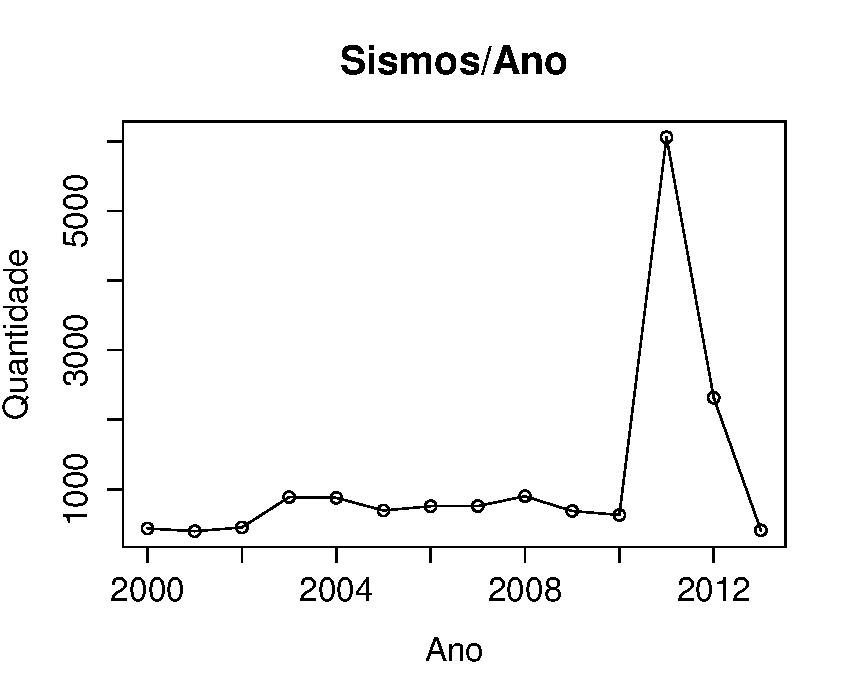
\includegraphics[scale=0.9]{img/ocorrenciasAno.pdf}
\caption{Amount of earthquake by year.}
\label{ocorrenciasAno}
\end{figure}

Based on the statement done before and considering that we want earthquakes that follow more stable patterns, we selected the ones that happened in land areas or very shallow sea areas, with maximum depth of 100 kilometers and magnitude above 3.0 in the Richter Scale.\\

For the experiments, the data was changed into slices for every year. Each slice is as follows: if the base contains data about a time interval of 10 years, it will be split in 10 slices.\\

We also selected some sub-areas in Japan to better extract and understand earthquakes characteristics and patterns. Those areas are Kanto, Kansai, Touhoku and East Japan. The Figure~\ref{alljapan} shows how we defined them. They are discribed as follows:

\paragraph{Kanto} Kanto is the region around Tokyo. It is area with high simologic activity during the years we studied. Its coordenates are 34.8 North, 138.8 West, with  2025 bins. Each bin covers an area of approximately 25km$^2$.\\

\paragraph{Kansai} Kansai is the region that includes Kyoto, Osaka and many others historical cities. In this area, rather than Kanto area, there is a small sismic activity. Its coordenates are 34 North, 134.5 West, with 1600 bins. Each bin covers an area of approximately 25km$^2$.\\

\paragraph{Touhoku} Touhoku is the region in the North of the main japanese island. It has some clusters of sismic activities during the the years we studied. Its coordenates are 37.8 North, 139.8 West, with  800 bins. Each bin covers an area of approximately 100km$^2$. \\

\paragraph{East Japan} Is the region that is related with the east coast of Japan. It is the most different area, because it has eathquakes that happend both in land or in the sea. It was in this region that the 9.0 $M_w$ earthquake happened. Its coordenates are 37 North, 140 West, with 1600 bins. Each bin covers an area of approximately 100km$^2$. \\

\begin{figure}[!htb]
\centering
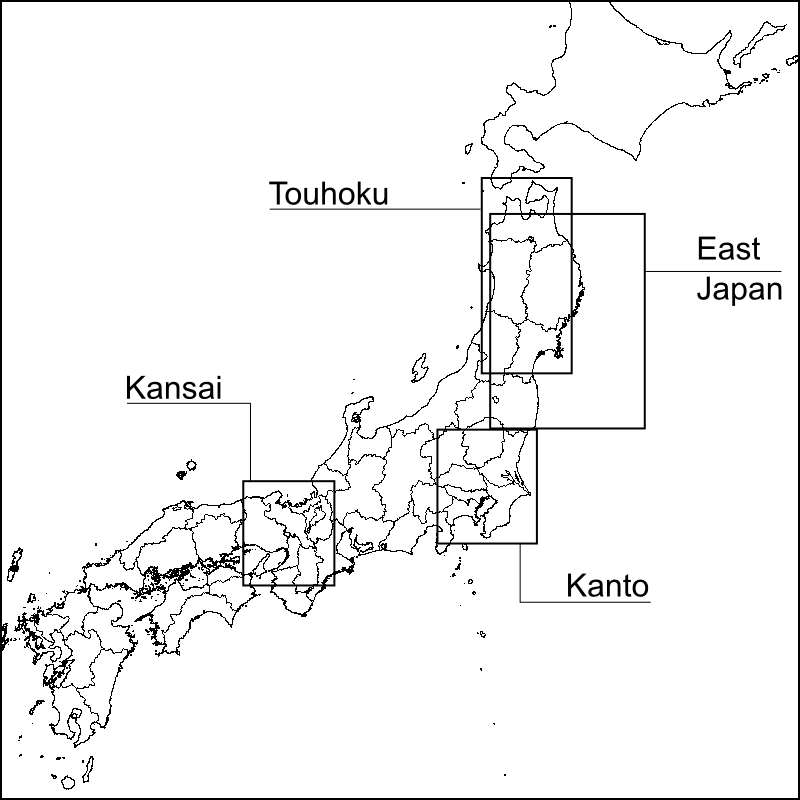
\includegraphics[scale=0.5]{alljapan.png}
\caption{Japan and the areas used in this studied.}
\label{alljapan}
\end{figure}

